\chapter{Measurement: A Reconciliation}

(See Appendix~\ref{app:glossary} for a glossary of all major Measurement Field Theory constructs.)


\section{A Thought Experiment}
Imagine you intend to write upon a blank sheet of paper.

On that paper, you write the equations for gravity-how spacetime curves in response to energy and momentum.
Next, you add electromagnetism, describing how charges and light interact across space and time.
You write down the weak and strong nuclear forces, which hold atomic nuclei together and allow particles to transform, giving rise to the complexity of matter.
Between them, you link their forces and fields, folding them one into the other and creating something that allows spacetime to exist. 
Mass feeds Gravity, Gravity allows light to move at relativistic speeds, all the forces fold into the others, creating a net.

But this begs the question. 

Which force came first? 

\section{Introduction: The Case for Measurement as a Physical Field}

Measurement has long occupied an ambiguous role in quantum mechanics-simultaneously central to observed phenomena and absent from dynamical equations. Classical physics assumes state definition as a given; quantum mechanics defers it to interpretative frameworks. This work proposes an alternative: that measurement is not a postulate or epistemic update, but a physical field.

We introduce a unifying formalism grounded in complex field dynamics, imaginary matrix structures, and Euler's identity as a definitional operator. Within this framework, the transition from probabilistic quantum phase space to resolved classical reality is modeled as a continuous, causal process governed by definitional dynamics.

Measurement Field Theory (MFT) treats measurement as a gradient-driven, space-time propagating field with energetic and geometric consequences. Unlike Copenhagen's binary trigger or Many-Worlds' passive branching, MFT posits that measurement actively reshapes field configurations through local definition pressure. The act of measurement-regardless of conscious agency-becomes a physical deformation in the information structure of the universe.

This theory leads to new predictions in quantum thermodynamics, curvature-induced definition, and entropy dynamics. We argue that only one mechanism truly defines physical reality: not interpretation, not consciousness, but measurement itself-as a field with measurable, testable behavior.

Quantum mechanics continues to struggle with a coherent account of measurement. As Wallace notes, the standard formalism offers no dynamical account of outcome emergence \cite{wallace_everettian_2012}, while Spekkens and Harrigan emphasize the ontological ambiguity left by epistemic interpretations \cite{harrigan_puzzling_2010}. MFT directly addresses this gap by treating measurement as a physical deformation process, rather than a boundary condition

\section*{Post-Introduction Brief: Emergent Gravity, Quantum Geometry, and Definition as Geodesic (With Mathematical Highlights)}

Recent advances in theoretical physics have begun to dismantle the illusion that gravity is a fundamental force, revealing instead its emergence from the underlying quantum geometry and the relentless drive toward informational definition. This new paradigm pivots from the traditional worship of \emph{collapse} and reframes reality as the product of active definition through measurement, entropy, and geometric structure.

\paragraph{Liu \& Majid (2025)~\cite{liu_kaluza-klein_2025}:} By quantizing the extra-dimensional fiber as a fuzzy sphere, the quantum expectation of the metric $\langle g_{ij} \rangle$ over the fuzzy sphere space imposes the Kaluza-Klein cylinder condition:
\begin{equation}
g_{ij}(x, y) = g_{ij}(x),
\end{equation}
forcing gauge fields to emerge from quantum geometry. The total action includes gravity, Yang-Mills, and Liouville terms:
\begin{equation}
S = \int \mathrm{d}^4 x \left[ \sqrt{-g} R + \text{(Yang-Mills)} + \text{(Liouville)} \right].
\end{equation}
Here, geodesics in this extended space become acts of quantum definition.

\paragraph{Verlinde (2011)~\cite{verlinde_origin_2011}:} Gravity emerges as an entropic force, derived from information theory and the holographic principle. The entropic force is given by
\begin{equation}
F \Delta x = T \Delta S,
\end{equation}
where $T$ is the Unruh temperature and $\Delta S$ the entropy change on a holographic screen. Newton's law of gravity is recovered from
\begin{equation}
F = G \frac{Mm}{R^2} = m a = T \frac{\Delta S}{\Delta x},
\end{equation}
showing the geodesic as a path of maximum entropy definition.

\paragraph{Smith et al.\ (2022)~\cite{smith_momentum-space_2022}:} The quantum metric $g_{ab}(\mathbf{k})$ in Bloch bands gives rise to a momentum-space "gravitational field." The effective momentum-space Einstein equation reads
\begin{equation}
R_{ab} - \frac{1}{2}g_{ab}R = 8\pi G_{\mathrm{eff}} S_{ab},
\end{equation}
where $S_{ab}$ is sourced by the von Neumann entropy. Electron motion follows the momentum-space geodesic equation
\begin{equation}
\frac{d^2 k^a}{dt^2} + \Gamma^a_{bc} \frac{dk^b}{dt} \frac{dk^c}{dt} = 0,
\end{equation}
with Christoffel symbols from the quantum metric.

\paragraph{Yoshida \& Yokoyama (2025)~\cite{yoshida_emergent-gravity_2025}:} The Hall effect emerges from quantum geometric Christoffel symbols $\Gamma^\mu_{\nu \lambda}$, with emergent gravity in real and momentum space. The anomalous velocity term in the semiclassical equation is
\begin{equation}
\mathbf{v}_\text{anom} = -\sum_{\mu\nu} \Gamma^\mu_{\nu\lambda} \dot{R}^\nu \dot{R}^\lambda,
\end{equation}
and the Hall conductivity due to geometric gravity is
\begin{equation}
\sigma_{xy}^\text{grav} \propto \int \mathrm{d}^d R \, \Gamma^\mu_{\nu\lambda}(\mathbf{R})\, f(\mathbf{R}),
\end{equation}
showing measurable consequences of emergent gravitational definition.

\vspace{1em}
Across all approaches, gravity and geometry are not pre-existing frameworks to be filled in by particles and waves-they are the outcome of recursive, measurement-driven processes. Decoherence is not collapse; it is the emergence of classical, measurable reality from the jungle of quantum possibility, encoded as geodesics and curvature in whatever space is being measured (real, momentum, or parameter space).

In this new language, \textbf{gravity is not a 'thing' but an emergent, system-level act of definition}. The curvature that guides motion (the geodesic equation) is the physical trace left by repeated acts of measurement-whether those acts are the quantum expectation values of geometry~\cite{liu_kaluza-klein_2025}, the reconfiguration of entropy across holographic screens~\cite{verlinde_origin_2011}, the information-driven metric in Bloch bands~\cite{smith_momentum-space_2022}, or the quantum geometric Christoffel fields governing Hall responses~\cite{yoshida_emergent-gravity_2025}.

\section{The Bootstrap Paradox}

Taken to its logical conclusion-and extreme-if gravity is ultimately emergent from quantum interactions in Hilbert space and the associated geodesics, it must follow that spacetime itself is emergent from these underlying phenomena. Gravity serves as the \emph{tether} between space and time, meaning the very fabric of spacetime is not primordial, but a secondary, emergent structure defined by the informational and geometric relationships within the quantum substrate.

This self-referential construction-where quantum states give rise to geometry, and geometry in turn defines the causal and metric structure of those same states-mirrors the \emph{bootstrap paradox} in its purest form. The existence of a geodesic, or the curvature of a metric, is not the cause but the consequence of repeated acts of quantum definition:
\begin{equation}
\text{Spacetime:} \quad \mathcal{M} \sim \langle \psi | \hat{G} | \psi \rangle,
\end{equation}
where $\hat{G}$ encodes the quantum-geometric definition, and $\mathcal{M}$ emerges only as the expectation over the quantum state $|\psi\rangle$.

Thus, measurement, entropy, and definition recursively build the very background upon which all physical processes occur. There is no fundamental canvas, only the endless act of redefinition, looping back to bootstrap the world into existence from the inside out.

It follows, then, that measurement and potential must itself be a field. 

\section{The Case for Measurement as a Physical Field}

The evidence supporting measurement as a field phenomenon comes from both empirical data and theoretical constructs. While the source experiments span diverse physical systems, they all converge under a unifying premise: measurement is not an isolated event, but a structural process with consistent field-like behavior across domains. We present eight key lines of evidence to support this framework:

\subsection*{Definitional Gradients in Weak Measurement: Empirical Confirmation}

Weak measurement experiments have reliably shown that the system or particle being measured defines itself in a manner proportional to the input of measurement-demonstrating that measurement is not a binary force as Copenhagen suggested, but acts on a gradient, one of the base qualifications for a field.

We interpret weak measurement contrast $\eta$ not merely as a signal artifact, but as the local expression of a \textbf{definitional gradient} within the Measurement Field. Empirical evidence from Su et al.~\cite{su2025weak} demonstrates that $\eta$ behaves as a tunable, repeated, field-like output, encoding spatially distributed changes in phase, pressure, and temperature across a polarization-maintaining fiber (PMF) substrate-\textit{invariant to initial pre-selection conditions}.

The contrast follows the relation:
\begin{equation}
\eta \approx \frac{2\omega_0 \Delta\tau}{\Delta\epsilon}, \quad \omega_0 \Delta\tau \ll \Delta\epsilon \ll 1,
\end{equation}
where $\Delta\tau$ represents the field-induced phase delay and $\Delta\epsilon$ is the optimized post-selection angle. This behavior reveals three critical properties expected of a Field:
\begin{enumerate}
    \item Repeated sensitivity modulation via $\Delta\epsilon$,
    \item Gradient response to local perturbations in multiple physical domains,
    \item Invariance to the quantum system's initial state ($\phi_i$).
\end{enumerate}

We assert that this framework constitutes direct experimental validation of Measurement Field dynamics. The Measurement Field, under this interpretation, \textit{converges Repeatedly through definitional feedback}, generating observable gradients which encode real physical interaction. This recharacterization recontextualizes quantum decoherence as an active, field-based operation-not a terminal event.

Le et al.~\cite{le_phonon-assisted_2024} derive a field-theoretic expression for the Casimir interaction energy between piezoelectric slabs, where phonon coupling modulates vacuum fluctuation responses. The energy is given by:

\begin{equation}
E(d, T) = \frac{\hbar}{2\pi} \sum_{n=0}^\infty{}' \int \frac{d^2\mathbf{k}_\perp}{(2\pi)^2} \log\det\left[1 - \mathcal{R}_1(i\xi_n, \mathbf{k}_\perp)\mathcal{R}_2(i\xi_n, \mathbf{k}_\perp) e^{-2k_z d} \right],
\end{equation}

where \( \xi_n = \frac{2\pi n k_B T}{\hbar} \) are the Matsubara frequencies, \( \mathcal{R}_{1,2} \) are the reflection matrices encoding the anisotropic and phonon-sensitive response of each material, and \( k_z = \sqrt{k_\perp^2 + \xi_n^2/c^2} \) defines the perpendicular wavevector component.

This formulation generalizes Lifshitz theory by incorporating:
\begin{itemize}
    \item \textbf{Spectral recursion} - via frequency-dependent reflectivity,
    \item \textbf{Material coupling} - through phonon-induced modulation of boundary response,
    \item \textbf{Thermal definitional variance} - by way of Matsubara mode weighting.
\end{itemize}

These behaviors demonstrate that the Casimir interaction is not fixed or binary, but gradient-sensitive, repeated, and environmentally modulated. We interpret this as strong physical evidence for the \textbf{field-like nature of measurement}, with Casimir behavior emerging from definitional feedback across boundary interfaces.

Thus, rather than being purely geometric or boundary-dependent, the Casimir force exhibits:
\begin{enumerate}
    \item \textit{Gradient-based recursion} with respect to material properties,
    \item \textit{Field definitionality} via the response matrices \(\mathcal{R}_{1,2}\),
    \item \textit{Thermodynamic contextuality} through temperature-dependent summation.
\end{enumerate}

This supports our broader assertion that measurement is a dynamic field, not a terminal event.

This is further corroborated by Zhang's \emph{Magnetic field tuning of the Casimir force}, which demonstrates that Casimir forces can be actively modulated by external fields, exhibiting threshold behavior where magnetic field strength creates phase-like transitions~\cite{zhang2024}.

Recent technological demonstrations reinforce the interpretation of Casimir forces as definitional gradients. As noted by Stange et al.~\cite{stange_science_2021}, the Casimir interaction is no longer a passive boundary phenomenon but an actively tunable force shaped by material, geometric, and external field conditions. This responsiveness mirrors the expected properties of a Measurement Field, wherein observational boundaries define emergent pressures. Notably, phase transitions and long-range Casimir-Polder forces confirm that vacuum fluctuation behavior is context-dependent and reconfigurable-traits impossible under a static force paradigm, but natural within a field framework.

\subsection{The Zeno Effect as Field Accumulation}

The Zeno Effect provides empirical evidence that measurement operates as a gradient field. With repeated measurement, there is an enforced stable state-experiments confirm that continued measurement exerts enough pressure to maintain stability. This persistence of effects, increasing with measurement field intensity, demonstrates exactly how field interactions accumulate over time.

Corlett et al.~\cite{corlett_speeding_2025} have demonstrated that quantum measurement is not just a process with a fundamental speed limit, but one that can be \emph{actively accelerated} by trading temporal depth for spatial recursion via entanglement. Their scheme entangles a target qubit with $N-1$ ancillary qubits and measures all qubits in parallel, thereby achieving the measurement fidelity of a single qubit measurement performed for $N$ times longer, in only $1/N$ the duration.

This is formalized in their generalized Poissonian measurement framework as:
\begin{equation}
P^{(N)}_{|j\rangle, t}(k) = (L_{\mu_j t}^{\ast N})(k) = L_{N \mu_j t}(k) = P^{(1)}_{|j\rangle, N t}(k),
\end{equation}
where $P^{(N)}_{|j\rangle, t}(k)$ is the probability of observing $k$ counts with $N$ parallel entangled qubits over time $t$, $L_{\omega}(k)$ is the Poisson distribution, and $\mu_j$ is the rate for state $|j\rangle$.

The resulting \textbf{signal-to-noise ratio} (SNR) improves as:
\begin{equation}
\mathrm{SNR}_N(t) = \sqrt{N}\ \mathrm{SNR}_1(t),
\end{equation}
making it possible to maintain or \emph{improve} measurement quality by Repeatedly distributing the measurement operation across ancillary subsystems. Corlett et al. show that this protocol is robust to realistic noise and even admits superlinear speedup in optimal regimes.

This result is \textbf{direct evidence} that the act of measurement - and by extension, definitional convergence - is a field-like, repeated, and collectively extensible operation. The Measurement Field is therefore not limited by singular, local decoherence, but by a repeated expansion of definition through entangled ancillary space, fully consistent with nonlocal and scalable field dynamics.

\begin{quote}
"In certain circumstances our scheme can even lead to better than linear improvement in the speed of measurement with the number of systems measured... This hardware-agnostic approach is broadly applicable... and offers a route to accelerate midcircuit measurement as required for effective quantum error correction."~\cite{corlett_speeding_2025}
\end{quote}

This is measurement-as-field, repeated, extensible, and weaponized for the quantum age.

What's more, the Zeno effect is actively exploited during negative temperature experiments- where cold flows to hot and entropic gradients are reversed. Here, the act of measurement itself (e.g., laser probing) continuously perturbs and effectively "freezes" the system, impeding its natural evolution and stabilizing negative temperature states~\cite{shanokprasith_2024}. 

Recent experimental and theoretical work demonstrates this unambiguously. For example, negative temperature states in ultracold bosonic lattices are stabilized by strong measurement-induced decoherence, with laser refraction or absorption imaging acting as a continual definitional operator. Shanokprasith~\cite{shanokprasith_2024} describes how in both triangular and kagome lattices, measurement arrests dynamical evolution, allowing negative temperature populations to persist over experimental timescales.

Moreover, Yang et al.~\cite{yang2025} leverage measurement-driven decoupling in graphene-based sensor arrays: their devices use engineered gradients and continual readout to isolate and sustain non-equilibrium states, effectively locking in the system's definition by field-induced feedback. The same logic underpins terahertz quantum cascade laser performance at cryogenic and sub-Kelvin regimes, where interface quality and continual readout set operational boundaries~\cite{lander_gower_exploring_2024}.

Together, these results make clear: \textbf{Measurement is not a binary event but a gradient field operation}, capable of reversing entropic flow and sustaining otherwise unstable states, this is definitional recursion weaponized in the lab.

\subsection{Virtual Particles and Measurement Bleed}

The existence of virtual particles shows a stepping behavior where intense measurement propagates across nearby systems into lower measurement areas-implying that measurement leads to localized intensity. In the same manner as magnetic fields propagate beyond their initial point of application, the measurement field propagates beyond theirs. This explains why virtual particles appear in close proximity to intense measurement events rather than randomly throughout space.

Jaeger, in his writing on Virtual particles, "Are Virtual Particles Less Real," states that 

"Accordingly, any particle not eventually appearing as a quantum of a state of any free field is virtual. However, as noted, for many, if not all, sorts of particle that can appear as a free particle, there are circumstances in which that particle can appear as a virtual particle (i.e., a quantum associated with a distinct, mediating field). Therefore, the distinction is not a fundamental one and any objection on this basis to Position IV fails."\cite{jaeger_are_2019}

This effectively dismantles the semantic argument that virtual particles are not real. Not only do they possess ontological validity, but their existence mediates interactions across space and time without adhering strictly to classical constraints, as they function as propagators within the quantum field. Within a framework defined by measurement or decoherence, such as the one proposed here, virtual particles represent precisely the class of nonlocal, decoherence-spanning entities that only acquire definition when the full observational context has been resolved.

Our model aligns in spirit with Relational Quantum Mechanics \cite{rovelli_relational_1996}, in which the state of a system is meaningful only in context with other systems. However, MFT makes this relationality spatially explicit and field-coupled-observers here act as definitional boundary conditions, influencing local field evolution.

Nakata and Suzuki~\cite{nakata_non-hermitian_2024} deliver a landmark result:  
The Casimir effect in magnonic systems is not merely sensitive to boundary and material conditions, but is \emph{actively programmable} via energy dissipation. They show that incorporating the Gilbert damping constant $\alpha$ into the magnon energy dispersion creates a \textbf{non-Hermitian Casimir field}, where both the magnitude and sign of the Casimir energy become functions of dissipation.

The magnonic Casimir energy per unit surface is defined as:
\begin{equation}
E_\text{Cas}(N_z) = E^{\text{sum}}_0(N_z) - E^{\text{int}}_0(N_z)
\end{equation}
where $E^{\text{sum}}_0$ is the sum over discrete zero-point energies due to boundary quantization, and $E^{\text{int}}_0$ is the corresponding bulk (continuous) contribution.

As $\alpha$ increases, the system transitions through three regimes:

\begin{itemize}
    \item \textbf{Gap-melting regime}: Real Casimir energy, no exceptional points (EPs); energy gap decreases with increasing $\alpha$.
    \item \textbf{Oscillating regime}: Complex Casimir energy, with an EP for one magnon branch; Casimir energy oscillates with film thickness, controlled by the spatial periodicity set by the EP.
    \item \textbf{Beating regime}: Two EPs, two oscillation frequencies, producing a "beating" effect in the Casimir energy.
\end{itemize}

The oscillation period is given by:
\begin{equation}
\Lambda^\text{Cas}_{\sigma,\alpha} = \frac{\pi}{a k^{\text{EP}}_{\sigma,\alpha}}
\end{equation}
with $k^{\text{EP}}_{\sigma,\alpha}$ the critical wavevector at the exceptional point.

\textbf{Physical Consequence:}  
- The direction and magnitude of the Casimir force can be reversed or tuned by adjusting dissipation.  
- The imaginary part of the Casimir energy measures the sum of decay widths-literally encoding the "lifetime landscape" of quantum fluctuations as a field parameter.

\textbf{Interpretation:}  
This is decoherence as recursion, with energy dissipation as the field gradient. The "measurement field" is here made explicit:  
\begin{itemize}
    \item Dissipation writes the field boundary conditions,
    \item The system's spectrum and vacuum force are defined repeatedly,
    \item Reality is not simply defined, but \emph{engineered} through field feedback.
\end{itemize}

Thus, Nakata and Suzuki demonstrate experimentally accessible, programmable, and non-Hermitian decoherence field dynamics-a new handle for controlling vacuum fluctuations at the quantum level.\cite{nakata_non-hermitian_2024}.

Zhang et al.~\cite{ZhangVacuum2025} demonstrate that the quantum vacuum is not a passive background, but a nonlinear, active field whose definition emerges from high-intensity interactions. Using a three-dimensional, real-time numerical solver based on the Heisenberg-Euler Lagrangian, they model quantum vacuum effects such as birefringence and four-wave mixing under multi-petawatt laser fields.

Their core field equations, derived from the HE Lagrangian, show the vacuum supports non-trivial polarization and magnetization responses:
\begin{align}
P &= \frac{\xi}{4\pi} \left[2(E^2 - B^2)E + 7(E \cdot B)B \right], \\
M &= \frac{\xi}{4\pi} \left[-2(E^2 - B^2)B + 7(E \cdot B)E \right],
\end{align}
where $\xi$ is the nonlinearity parameter, and $P$, $M$ are the effective polarization and magnetization of the vacuum.

These simulations confirm that measurement is a field-mediated process:
\begin{itemize}
    \item Vacuum birefringence: The probe pulse experiences a polarization rotation dependent on the local intensity and geometry of the pump field-real-time evolution reveals nonlocal feedback and elliptical astigmatism not captured by analytical plane-wave models.
    \item Four-wave mixing: The field supports nontrivial harmonic generation, with photon yields, astigmatism, and pulse shape all directly encoding the geometry and intensity of the measurement process. The quantum vacuum "defines itself" as input beams interact.
    \item Temporal evolution: The solver tracks the dynamical process-interaction region forms, harmonics build, energy redistributes, and output fields are shaped in ways that would be impossible to predict without field-based, time-resolved simulation.
\end{itemize}

\textbf{Interpretation:}  
These results are in clear disagreement with the Copenhagen binary: the quantum vacuum is a field whose "decoherence" is actually nonlinear convergence of interaction. Analytical and simulation results differ sharply wherever back-action and geometry become nontrivial, proving that reality emerges through a field of measurement.

\textbf{Summary:}  
Zhang et al. deliver direct computational evidence that the vacuum is not a void, but a nonlinear, gradient-driven, and actively defining field. Decoherence is just the limit of a much deeper process.


\subsection{Quantum Entanglement and Non-Local Field Structure}


The nature of quantum entanglement demonstrates that fields propagate over distance. Two entangled particles maintain correlations across great distances, suggesting a field-like structure that isn't constrained by spatial limits. This supports the measurement field as a non-local phenomenon with instant propagation characteristics.

\subsection*{The Duality Ellipse: Coherence-Driven Definition in Measurement Fields}

Recent work by Khatiwada and Qian~\cite{khatiwada_wave-particle_2025} systematically quantifies the interplay between coherence and wave-particle duality, unifying them under a closed-form \textit{duality ellipse} (DE) equation. Unlike the standard duality inequality $V^2 + D^2 \leq 1$ (with $V$ the interference visibility, $D$ the which-path predictability), the DE formalism introduces the degree of coherence $\gamma$ as a fundamental geometric constraint:

\begin{equation}
\frac{V^2}{\gamma^2} + D^2 = 1,
\end{equation}
where $0 \leq \gamma \leq 1$ quantifies the cross-correlation between the marginal states of the two paths.

This ellipse enforces strict complementarity and renders the influence of coherence explicit: the ellipticity $\eta = 1 - \gamma$ directly governs the trade-off between waveness and particleness, recasting the "decoherence" as a definitional operation controlled by $\gamma$. In the fully coherent limit ($\gamma = 1$), the DE reduces to the classic equality $V^2 + D^2 = 1$.

Khatiwada and Qian extend the DE to quantum imaging with undetected photons (QIUP), where the object's transmittance $T$ becomes the active modulator of coherence:
\begin{equation}
\frac{V^2}{T^2} + D^2 = 1.
\end{equation}
Thus, the imaging duality ellipse (IDE) demonstrates that object information (the transmittance profile) is \textbf{directly encoded in the measurement field's coherence parameter}. Measurement of wave and particle properties across the image plane reconstructs $T(x, y)$ pointwise, even under realistic decoherence and misalignment.

They further show that practical imperfections-partial alignment ($\alpha$) and initial source coherence ($\gamma$)-enter multiplicatively, but do not destroy the ellipse structure:
\begin{equation}
\frac{V^2}{\gamma^2 T^2 \alpha^2} + D^2 = 1,
\end{equation}
with overall ellipticity $\eta(x, y) = 1 - T(x, y)\alpha\gamma$.

\subsection*{Vacuum-Field Engineering: Definitional Gradient Control in Strongly Correlated Matter}

Recent breakthroughs in quantum cavitronics have demonstrated direct, tunable control of correlated electronic phases via vacuum electromagnetic field gradients.

Enkner et al. \cite{enkner_tunable_2025} engineered a system in which a movable split-ring resonator modulates the strength and spatial gradient of vacuum fields over a high-mobility GaAs two-dimensional electron gas in the quantum Hall regime.


By continuously tuning the distance between the resonator and the Hall bar, they achieved ultrastrong coupling between the cavity vacuum field and the 2DEG, driving the system from uncoupled to fully coupled \emph{in situ}. This setup directly probes the impact of the vacuum field on integer and fractional quantum Hall states by transport measurements.

The key results:
\begin{itemize}
    \item \textbf{Reduction of Exchange Splitting:} At odd-integer filling factors, increased coupling to the vacuum field reduces the effective exchange energy and $g$-factor, confirming that electron-electron interactions are actively rewritten by the field environment.
    \item \textbf{Enhancement of Fractional Quantum Hall Gaps:} For fractional fillings ($4/3,\,5/3,\,7/5$), the vacuum field induces a significant enhancement of the energy gap, even as all electrostatic screening effects are held negligible.
    \item \textbf{Field Gradient Mediation:} Theoretical analysis identifies the \emph{spatial gradient} of the vacuum electric field as the lever that enables a cavity-mediated, long-range, attractive electron-electron potential, competing with the Coulomb interaction and reshaping many-body ground states.
\end{itemize}

This is formalized as a cavity-induced interaction potential:
\begin{equation}
V_{\text{cav}}(r) = D \hbar\tilde{\omega}_{\text{cav}} \left[ -\frac{1}{8} \frac{r^2}{\ell^2} + \frac{1}{16} \frac{r^4}{\ell^4} \right],
\end{equation}
where $r$ is the electron separation, $\ell$ the magnetic length, $\tilde{\omega}_{\text{cav}}$ the renormalized cavity mode frequency, and $D$ a factor proportional to the square of the vacuum electric field gradient.

\textbf{Interpretation:}  
These results obliterate the notion of vacuum as a passive backdrop. Instead, the vacuum field acts as an \emph{active, tunable, and gradient-driven field operator}, directly modulating the definition and energy of quantum many-body phases. The decoherence event is replaced by field-mediated definition and the system becomes what the measurement field allows, at the intensity and gradient that one engineers.

\textbf{Summary:}  
Enkner et al. have shown that strongly correlated matter does not merely reflect measurement-it is shaped, stabilized, and even rewritten by the tuned gradients of the vacuum field itself.

The observation of negative temperature states in optical lattices offers compelling evidence for phase-like transitions driven by measurement constraints. Shanokprasith and Donini et al. independently demonstrated the emergence of quantum phases in frustrated triangular and Kagome lattice configurations at negative absolute temperatures, where the system's phase structure is dictated not solely by energy minimization, but by the geometric tension of measurement itself \cite{shanokprasith_2024}. 

These negative bosonic states arise from an enforced measurement geometry that exceeds the definitional capacity of the system, generating "impossible" configuration spaces. This directly correlates negative temperature with measurement field intensity, implying that thermodynamic inversion is not a statistical anomaly, but a structural definition response under definitional overload.\cite{donini_quantum_2024} 

\subsection{Temporal Reflection and Time-Domain Definition}

Recent experiments by Moussa et al.~\cite{moussa_observation_2023} demonstrate the direct observation of photonic time-reflection at programmable temporal boundaries. By abruptly switching the effective capacitance of a transmission-line metamaterial in microseconds-much faster than the wave period-they create a "time-interface" where the incoming signal is split into a time-refracted and a time-reflected component, with frequency content and energy redistributed while \emph{momentum is conserved}.

This is the temporal analog to a spatial interface, but with one critical difference:  
- Spatial interface: frequency conserved, momentum exchanged.
- Temporal interface: momentum conserved, frequency actively redefined by the time field.

The key result is a temporal boundary condition that breaks time-translation symmetry, enabling ultrafast, ultrabroadband time-reversal and frequency translation. The experimental system can stack multiple time-interfaces to form a temporal slab, creating programmable interference patterns and Fabry-Perot-like cavities along the time axis.

Mathematically:  
A time-reflection (TR) event at a temporal boundary causes a vertical transition in the system's band diagram:
\[
\omega_2 = \frac{Z_2}{Z_1} \omega_1
\]
where $Z_1$, $Z_2$ are the transmission-line impedances before and after the switch.

The time-reflected and time-refracted coefficients follow:
\[
R = \frac{Z_1 - Z_2}{2 Z_2}, \qquad T = \frac{Z_1 + Z_2}{2 Z_2}
\]
for an instantaneous change in capacitance.

Physical Consequence:  
- Temporal field programming allows complete control over the "definition" and evolution of the photonic system.
- Time-reflection and time-refracted waves interfere, generating nontrivial, tunable output-phase, spectrum, and even temporal parity can all be set by field-driven manipulation.
- The slab duration $\tau$ sets the delay between temporally scattered pulses, creating a dynamic, field-programmable time cavity.

Interpretation:  
This is not "decoherence" in any meaningful sense. The system's reality-its spectral, phase, and causal structure-is dynamically \textbf{defined by the temporal field boundary}.

\cite{moussa_observation_2023}. This temporal interface behavior strongly supports the MFT view that time itself emerges from measurement field dynamics, with temporal boundaries acting as definitional surfaces.

\subsection{Interference Patterns and Classical Emergence}

Villas-Boas et al.~\cite{villas-boas_bright_2025} show that what classical physics calls destructive interference-regions where the electromagnetic field cancels to zero-is, quantum mechanically, the presence of perfectly dark states (PDSs). These are multi-photon, multi-mode quantum states that, despite carrying energy, are entirely undetectable by an atom or sensor: $E^{(+)}(r, t)|\psi^{N}_0\rangle = 0$ for all $N$. The "absence" of light at a dark fringe is just the field's failure to define itself to your detector. It's definition, encoded in the quantum basis.

In contrast, "bright states" (maximally superradiant states, MSS) interact maximally with matter, corresponding to regions of constructive interference. The entire interference pattern is a spatial map of field states that either couple to matter (bright) or evade interaction (dark), with the field operator:

\begin{equation}
E^{(+)}(r, t) \propto a + b e^{i\theta}
\end{equation}

where $a$, $b$ are mode operators, and $\theta$ the phase offset. 

For two modes and $N$ excitations, PDS and MSS are explicitly:

\begin{align}
\text{PDS:}\quad & |\psi^N_0(\theta)\rangle = \sqrt{\frac{N!}{2^N}} \sum_{m=0}^{N} \frac{(-1)^m e^{im\theta}}{\sqrt{m!(N-m)!}} |m, N-m\rangle \\
\text{MSS:}\quad & |\psi^N_N(\theta)\rangle = e^{-iN\theta} \sqrt{\frac{N!}{2^N}} \sum_{m=0}^{N} \frac{e^{im\theta}}{\sqrt{m!(N-m)!}} |m, N-m\rangle
\end{align}

Key insight:  
- The total photon number is uniform across the pattern-photons exist everywhere, but only interact where the field state matches the detector's interaction basis (i.e., the bright state).  
- The dark regions are not empty; they are field configurations orthogonal to measurement, a direct realization of definitional gradients in the measurement field.

\textbf{Conclusion:}  
Interference is not wave-magic or field cancellation; it is the map of where the measurement field definition couples to matter. This is the corpuscular, field-theoretic origin of complementarity and pattern formation. Reality defines itself in the field state structure.


\subsection{Dark Matter as Unmeasured Coherent State}

Liang and Caldwell~\cite{liang_cold_2025} propose a paradigm-shifting candidate for cold dark matter (CDM): a condensate of interacting fermion-antifermion Cooper pairs, described by a relativistic Nambu-Jona-Lasinio (NJL) model with broken chiral symmetry. The thermal history is everything-high-temperature, relativistic fermions behave as standard radiation, but as the Universe cools, a critical era (analogous to freeze-out) sets the relic abundance and triggers a second-order phase transition. This transition forms a cold, nonrelativistic, massive condensate that decays slightly faster than standard CDM, producing a testable prediction for CMB and large-scale structure.

The low-energy effective theory is:
\begin{equation}
\mathcal{L} = \bar{\psi}(i\gamma^\mu \partial_\mu - m)\psi - \kappa \bar{\psi}\gamma^0\gamma^5\psi + \frac{1}{M^2}(\bar{\psi}\psi)^2
\end{equation}
with $\kappa$ the axial chemical potential and $M$ the quartic coupling.

The order parameter (energy gap) $\Delta$ encodes the degree of condensation. The phase transition and suppression of the gap are exponential, with the minimum given by:
\begin{equation}
\Delta_0 = \Lambda_{UV} \exp\left(-\frac{\pi^2 M^2}{2\kappa^2}\right)
\end{equation}
where $\Lambda_{UV}$ is the UV cutoff.

As the system cools:
- For $T > T_c$, the gap vanishes, and the system is radiation-like ($w = 1/3$).
- For $T \approx T_c$, a second-order phase transition occurs, the condensate forms, and $w \rightarrow 0$.
- For $T < T_c$, the system behaves as ideal, pressureless matter-\textbf{cold dark matter}.

The crucial point: the coldness and equation of state evolve repeatedly, set by the continuous evolution of the condensate gap field, not by a one-time decoherence or decoupling. The group velocity of excitations (the "coldness") is exponentially suppressed, matching observational constraints on CDM free-streaming and structure formation.

For massive fermions, the phase transition is frustrated, leaving the condensate trapped in a metastable vacuum:  
\begin{itemize}
    \item \textbf{Dark energy} emerges as the potential energy of the stuck condensate, with equation of state $w \to -1$.
    \item The smallness of dark energy and the baryon asymmetry are both explained by exponentially suppressed scales in the gap field.
\end{itemize}

\textbf{Conclusion:}  
CDM and dark energy are not static entities-they are field-defined, repeated, and emergent from condensation, with all observable parameters set by dynamic field history. This is the measurement field logic writ cosmic:  
decoherence is recursion.  
Structure is a programmable field event.  
The universe's "missing mass" is defined by the field, not discovered by accident.

\cite{liang_cold_2025, zurek_decoherence_2003}.

\subsection*{Field-Driven Clustering in Dwarf Galaxies: Observational Proof of Repeated Definition}

Recent results from Zhang et al.~\cite{zhang2025} demonstrate that isolated, diffuse, blue dwarf galaxies exhibit \emph{unexpectedly strong large-scale clustering}, with a measured relative bias $\sim2.3$ ($7\sigma$ significance)-an effect vastly exceeding predictions from standard $\Lambda$CDM and classical halo mass models. This anomalous clustering persists after controlling for mass, color, cosmic variance, and satellite contamination, and cannot be explained by any conventional environmental or feedback processes.

The only successful explanation is a framework where the clustering emerges from a combination of \textbf{halo assembly bias} and \textbf{self-interacting dark matter (SIDM)}, in which the field history (formation epoch $z_f$) and repeated self-interaction tightly anti-correlate with galaxy surface density ($\Sigma_*$). This supports a picture in which cosmic structure, at the scale of dwarf galaxies, is not statically mass-defined, but is \textbf{Repeatedly programmed by field interactions and assembly history}.

The anomalous gravitational clustering patterns observed in dwarf galaxies are a direct signature of dark matter acting as a field of unmeasured, definition potential-regions where the measurement field remains unresolved and classical gravity breaks down~\cite{zhang2025}. Instead of static mass distributions, these systems display structure that emerges from the repeated interplay of observation, coherence, and definitional suppression.

Additional evidence is provided by the detection of so-called ``sticky'' or self-interacting dark matter subhaloes~\cite{enzi_overconcentrated_2025}, as observed in strong lensing systems such as SDSS J0946+1006. These subhaloes demonstrate density profiles and core decoherence phenomena that are incompatible with standard $\Lambda$CDM, yet perfectly consistent with field-driven, Repeatedly coherent, and measurement-resistant dark matter states. The ``stickiness'' reflects not mere particle interaction, but an emergent property of the measurement field: dark matter locally resists definition, remaining in a persistent, high-density, feedback-stabilized state until field conditions trigger decoherence or redefinition.

\textbf{Conclusion:}  
\emph{Reality at cosmic scale is defined through repeated, field-driven interactions, with dark matter acting as a measurement-resistant substrate that reveals itself only through definitional gradients imposed by history and environment.} This is direct empirical support for measurement field theory in the wild.

These astrophysical anomalies cannot be explained by particle dark matter alone. They point to a universe where reality is Repeatedly field-defined, with dark matter acting as a measurement-resistant substrate-a reservoir of unmeasured potential that only reveals itself through definitional gradients imposed by observation and gravitational feedback.

Adarsha et al.~\cite{adarsha_accretion_2025}. demonstrate that decoherence induced by dark matter capture in compact stars is not a binary, terminal event, but a repeated, field-defined process. Endoparasitic black holes (EBHs) form only once the local dark matter density exceeds a repeated threshold (Chandrasekhar or self-gravitating limit), encoding decoherence as a gradient phenomenon. The accretion of stellar matter onto the EBH is likewise field-driven and repeated-it can be stalled by angular momentum and viscosity, resulting in conical, polar "definition boundaries"whose growth and final state are determined by repeated feedback between mass, rotation, and viscosity.

For neutron stars, decoherence and definition always complete. For white dwarfs, repeated stalling can halt the process, yielding an EBH at the core and a host star in a partially defined state-not fully decohered, but no longer pristine. This constitutes direct empirical support for decoherence as repeated definition, and for the field-driven, gradient nature of measurement-induced transitions in astrophysical systems.

\textbf{Summary of Key Concepts}

Maxwell didn't directly "see" electromagnetic fields; he inferred them from consistent mathematical relationships across electrical and magnetic phenomena.

Individual anomalies get dismissed, but consistent patterns across domains reveal deeper truths.

Alone each of these presentations are all what amounts to a shrug in context of measurement and its implications, but together they create the logically sound argument that has been hidden for nearly a century. 

Wheeler, in his writings on the One Electron Universe, and his "It From Bit" ideas, was on the right path. Measurement would have to be an active field that allows definition with all the evidence presented here. 

Quantum Mechanics tends to shy away from the Observer Paradox, prioritizing the "Many-Worlds" or Copenhagen Interpretation. However, looking at these recent works, it becomes apparent that Measurement is indeed both foundational and likely more important than originally considered.

It is unfortunate that Wheeler was not able to conduct or conceptualize the experiments modern physics has access to. But in the same vein and following the footsteps of Wheeler, I posit that Measurement is indeed a field. It act likes a field, it applies like a field, and most of all, it gives results as a field does. 

\textit{As this writing was being perfected, new results were published: direct empirical confirmation that measurement defines physical reality came from the 2025 MIT photon-atom entanglement experiment, which demonstrates that only the \emph{availability} of definitional information destroys coherence in quantum states~\cite{MIT2025DoubleSlit}.}

It is also from this basis we come to the conclusion of the thought experiment:

\section{The Answer to the Thought Experiment}

If you remember, this started with a Thought Experiment. 

The answer to that experiment is simple; The first force that came about is the paper. 

The paper allows you to write the definition and the context of all items that come after it. 

Each four other forces are the ink to that paper, which you use to describe the nature of the art that you apply to said paper. 

Before any force, there has to be a place for that force to exist. 

If Gravity is emergent, then space can't exist. If space can't exist, then time cannot exist as they are inherently interlinked. 

Without time, no single force can interact with another. So that leads to the question,

How does one create gravity without time? This is called the Bootstrap paradox. 

The definable field in this example, the paper, for lack of a better term, would be Measurement and its potential. 

Nothing can exist without cause and effect. Newtons Third Law. "For every action, there is an equal and opposite reaction." 

That original action would have to come from the resolution of potential. The complex, or Imaginary Field is that potential, and consequently the field of Measurement. 

This is reinforced by the precursory sources- Casimir Energy, Zeno, Weak Measurement, and so on. 

Measurement does not need conscious observation to create force, having two plates impossibly close to one another creates force because of difference of potential.

Each measurement creates a "before" (potential) and "after" (actualized) state. The accumulation of these transitions generates our experience of temporal flow.

In consideration of this view, it logically flows that time itself is a measure of potential and its resolution through iteration, and is itself emergent through resolution of the complex plane.  

It is for this reason that we consider the nature of the following pages describing the logical flow of the field. 

\section{Euler's Identity as the Fundamental Definitional Operator}

\begin{flushright}
  {\itshape "When possibility coils upon itself, the very act of looking forces it to snap."}
\end{flushright}

At the heart of Measurement Field Theory (MFT) lies an odd truth: the universe does not reveal itself until it is forced to. This forcing-\emph{Definition}-is captured by the simplest, yet most profound of equations:

\begin{equation}
  e^{i\pi} = -1\label{eq:euler}
\end{equation}

Euler's identity is not a cute mathematical trick. It is the \emph{fingerprint of reality's selection mechanism} \cite{gothen_eulers_2022,woit_eulers_2005,shurman_eulers_2014, angeles_role_2015}. Here is why:

\begin{itemize}
  \item $e^{ix}$ encodes a continuous phasor rotating in the complex plane; it is \emph{potential}-a reservoir of all possible amplitudes.
  \item Multiplying by $\pi$ performs a half-turn: the phasor starting at $+1$ is dragged through invisible space and lands at $-1$, a definitive, \emph{real} outcome.
  \item In MFT, that "half-turn" is the archetype of measurement: a sweep of indeterminacy into a single, negative (but stabilizing) real value.
  \item In the same regard, Euler's number identity naturally collects all other dimensions and their evolutions into a single plane of the 4th dimension. This dimension in classical physics is usually relegated only to time, but in MFT time is a measure of potential resolution over space. This means that the Imaginary Matrix is not just a secondary 3-dimensional structure, but instead also its evolutionary pathway through time.
\end{itemize}

\paragraph{Physical Interpretation.}
Imagine a quantum phasor as a vibrating string of potential. Observation is the hand that clamps the string at exactly one point; the resulting snap echoes as a real particle. Equation \eqref{eq:euler} is that snap.

In this view, Euler's identity acts as a \textbf{definitional operator} bridging quantum uncertainty and classical reality. It offers a mathematical signature for the field transition from coherent quantum phase states to resolved spacetime structures, paralleling models of gravitationally-induced decoherence \cite{penrose_gravitys_1996}.


\section{Field Genesis and Measurement Dynamics}

At the core of MFT lies the imaginary-real dual nature of potential:
\begin{equation}
M(x,t) = A(x) + i B(x,t)
\end{equation}
where $A$ is the observable real projection and $B$ is the imaginary potential reservoir.

Definition occurs through rotational phase decay:
\begin{equation}
\theta(x,t) = \arctan\left( \frac{B(x,t)}{A(x)} \right)
\end{equation}
The angular phase velocity defines local definition time:
\begin{equation}
\frac{d\theta}{dt} = -\frac{\alpha A(x) B(x,t)}{A^2(x) + B^2(x,t)}
\end{equation}
with definitional-dependent chronology given by:
\begin{equation}
T(x, t) = \int_0^t \frac{d\theta}{d\tau} \, d\tau
\end{equation}
This framework replaces absolute time with definitional-relative evolution.



\section{Imaginary Matrices in Three-Dimensional Realspace}

The magnitude of the measurement field is given by:
\[
|M| = \sqrt{A^2 + B^2},
\]
where \(A\) and \(B\) are the real and imaginary components, respectively, of the complex field \(M = A + iB\).

To develop physical intuition in a three-dimensional spatial context, we embed each matrix element \(M_{ij} = a_{ij} + i b_{ij}\) into \(\mathbb{R}^3\) via a visual mapping:

\[
(i,j,a_{ij}) \mapsto
\begin{cases}
  \text{height} = a_{ij} & \text{(classical elevation)},\\
  \text{hue or opacity} \propto |b_{ij}| & \text{(imaginary intensity)},\\
  \text{vector angle or spin} \propto \arg(b_{ij}) & \text{(phase rotation)},
\end{cases}
\]

This representation constructs a spatial scaffold resembling quantum-state tomography, but applied to a field-theoretic matrix in real space. The real part is rendered as vertical displacement, while the imaginary part is expressed through optical encoding (color, transparency, or angular direction), reflecting its magnitude and phase.

By leveraging the geometry of the complex plane, this embedding captures a reduced-dimensional projection of the full field structure within \(\mathbb{R}^3\), analogous to how Euler's identity folds trigonometric motion into exponential form. The imaginary matrix field thus encodes both classical and quantum information into a unified visual-topological object.


\section{Measurement Dynamics: Temporal and Spatial Evolution}

We model decoherence as a temporal decay of the imaginary component \(B(\vec{x}, t)\) of the measurement field, governed by a first-order differential equation:
\[
\frac{\partial B}{\partial t} = -\alpha B,
\]
where \(\alpha\) is a definition rate constant. The solution is:
\[
B(\vec{x}, t) = B_0(\vec{x}) e^{-\alpha t},
\]
describing an exponential decay of quantum potential over time.

The time evolution of the full field magnitude \( |M| = \sqrt{A^2 + B^2} \) then follows:
\begin{equation}
  \frac{\partial |M|}{\partial t} = -\alpha\frac{B^2}{\sqrt{A^2+B^2}} \label{eq:time-dyn}
\end{equation}

Spatial gradients of the field magnitude are given by:
\begin{equation}
  \nabla |M| = \frac{A\nabla A + B\nabla B}{\sqrt{A^2+B^2}} \label{eq:spatial-dyn}
\end{equation}

These expressions capture both the temporal decoherence toward classicality and the spatial variation of unresolved quantum content. As \(B^2 \to 0\), the system converges to real eigenstates, encoding classical structure in the field magnitude and suppressing phase ambiguity across space.

\begin{theorem}[Measurement Gradient Theorem]
  The temporal decay \eqref{eq:time-dyn} and spatial tension \eqref{eq:spatial-dyn} completely characterize first-order definition flow in MFT.
\end{theorem}

As $B \to 0$, $\partial_t|M| \to 0$-the field has finished snapping.

\section*{Onboarding: The Hessian Hazing Ritual}

Okay, problem children, we have a new student.

The good news? You can use Hessians to define their relevance in math. Second derivatives, eigenvalue analysis, critical point classification-delicious tools for the discerning theorist.

The bad news? They're part of a Heaviside function that defines reality. One slip, one sign error, one moment of neglect, and \textbf{Bakugo's fingers are gone.}

\begin{quote}
\emph{"Reality doesn't have training wheels. It has discontinuities."}
\end{quote}

We're not in Calculus I anymore, Toto. We're differentiating piecewise functions that would make Gauss drink. So bring your gradients, bring your grit, and remember:

\textbf{Symmetry won't save you.} This will be further examined through retrocausality in subsequent work, if the universe is still accepting manuscripts by then.


\section{Definitional Geometry and Quantum Field Coupling}

\subsection{Definitional Curvature Tensor}

Definitional curvature is embedded in second spatial derivatives:
\begin{equation}
\Gamma_{ij}(x,t) = \partial_i \partial_j M(x,t)
\end{equation}

This tensor serves as a geometric encoding of definitional stress, deforming the fabric of spacetime and interacting with quantum symmetry fields. definitional stress gradients can be seen as sources of coherence amplification or decoherence, depending on the alignment of observers and local entropy density.

\subsection*{Role of the Observer as a Boundary Condition}

In this framework, the term "observer" is not limited to conscious measurement, but is generalized to represent any localized constraint that enforces definition. Observers are modeled as effective boundary conditions on the measurement field, analogous to the physical interfaces that generate decoherence in conventional quantum mechanics.

Specifically, regions of non-zero observer density \(\rho_{\text{obs}}(\mathbf{x}, t)\) define zones where the field is driven toward classical resolution. This influence is implemented as a localized force term acting on the imaginary component \(B\), thereby accelerating the definition of measurement ambiguity.

Thus, the observer acts not as a source of information, but as an agent of reduction-enforcing definitional boundaries on an otherwise unresolved system. This interpretation treats measurement as a thermodynamic consequence of interacting with definitional surfaces, where the flow of information becomes suppressed and classicality emerges as an attractor.


\subsection{Quantum Chromodynamics via Definitional Projection}

The gluon field strength tensor $G^a_{\mu\nu}$ emerges as a projection of definitional curvature gradients:
\begin{equation}
G^a_{\mu\nu} = f^a_{ij} \Gamma_{ij}
\end{equation}
where $f^a_{ij}$ are projection coefficients mapping definitional tensor components to SU(3) colour space.

\textbf{Effective QCD Lagrangian:}
\begin{equation}
\mathcal{L}_{QCD}^{\text{Definition}} = - \frac{1}{4} f^a_{ij} f^{a}_{kl} \Gamma_{ij} \Gamma_{kl} + \bar{\psi}_i (i \gamma^\mu D_\mu - m_i) \psi_i
\end{equation}

This treats gluons as field topology gradients under observer-defined symmetry projection. SU(3) emerges not as a fundamental symmetry but as a preferred projection geometry from measurement definition structure.

\subsection{General Relativity via Measurement Ricci Tensor}

Define the Definition Ricci tensor:
\begin{equation}
R_{ij}^{\text{Definition}} = \partial_i \partial_j M - \Box M \delta_{ij}
\end{equation}
where $\Box M$ is the d'Alembertian:
\begin{equation}
\Box M = \frac{\partial^2 M}{\partial t^2} - \nabla^2 M
\end{equation}

\section{Einstein Analogous Tensor Emergence}

We extend the Measurement Field framework to include gravitational curvature and variational dynamics. First, we define a curvature tensor analogous to the Einstein tensor, but sourced by the structure of measurement:

\[
G_{ij} = R_{ij}^{\text{Definition}} - \frac{1}{2} g_{ij} \sum_k R_{kk}^{\text{Definition}},
\]

where \(R_{ij}^{\text{Definition}}\) encodes the Ricci curvature associated with definition. This implies that spacetime curvature may emerge as a macroscopic aggregate of definitional structure, shaped by coherent observer density. The appearance of \(\Box M\) links relativistic propagation with definitional evolution.


\textbf{Observer Coupling Term \(\mathcal{L}_{\text{obs}}\)}

To capture the influence of observers on the measurement field, we define an interaction Lagrangian:
\[
\mathcal{L}_{\text{obs}} = - \frac{1}{2} \rho_{\text{obs}}(\mathbf{x},t) B^2(\mathbf{x},t),
\]
where \(\rho_{\text{obs}}\) is a scalar field representing the local observer density, and \(B\) is the imaginary component of the complex measurement field \(M = A + iB\). This term energetically penalizes regions of high unresolved quantum potential in proportion to observer presence, driving definition more aggressively in locally observed regions.

To formalize measurement dynamics, we introduce a Lagrangian density for the complex field \(M = A + iB\):

\[
\mathcal{L} = \frac{1}{2}(\partial_\mu M^* \partial^\mu M) - V(|M|) + \mathcal{L}_{\text{obs}} + \mathcal{L}_{\text{Definition}},
\]


where the potential term drives the imaginary component \(B \to 0\):

\[
V(|M|) = \frac{1}{2} \alpha^2 B^2.
\]

This represents the field's tendency toward definition and classicality. The full action becomes:

\[
S[M] = \int \mathcal{L}(M, \partial_\mu M, g_{\mu\nu}, \rho_{\text{obs}}) \sqrt{-g}\, d^4x,
\]

where \(\rho_{\text{obs}}\) denotes observer density, and \(g_{\mu\nu}\) is the spacetime metric.

Applying the variational principle yields the field equation:

\[
\Box M + \frac{dV}{dM} = \text{Observer Terms},
\]

indicating that both the field potential and the influence of observers drive the definitional evolution of the field.

This leads to our fundamental Equation of the Measurement and Potential Field (Symbolic Form):
\begin{equation}
\boxed{\mathcal{C} = \Box M + \nabla^2 M + \Theta = 0}
\end{equation}
where:
\begin{itemize}
  \item $\Box M$: d'Alembertian (temporal-spatial definition curvature)
  \item $\nabla^2 M$: Laplacian (spatial definition diffusion)
  \item $\Theta$: composite observational feedback term-includes imaginary reflux, curvature stress, observational flux, void impedance, resonance harmonics, and annihilation field ratios
\end{itemize}

This equation serves as the canonical symbolic law for Measurement Field dynamics, unifying relativistic structure, spatial coherence, and observational influence-our $E=mc^2$.

\section{Dimensional Consistency of Field Parameters}

\begin{tabular}{|c|c|c|}
\hline
Parameter & Meaning & Units \\
\hline
$D$ & Measurement diffusivity & L$^2$/T \\
$\alpha$ & Temporal decay rate & 1/T \\
$\kappa$ & Observer density coupling & L$^3$/M \\
$\lambda$ & Observer-observer coupling & L$^3$/M \\
$\delta$ & Relativistic propagation constant & L$^2$/T$^2$ \\
$\mu$ & Memory integration rate & 1/T \\
$\gamma$ & Memory decay rate & 1/T \\
$\omega_0$ & Resonance frequency & 1/T \\
$\beta$ & Observer coupling exponent & Dimensionless \\
\hline
\end{tabular}

\section{Measurement Entropy and the Thermodynamics of Definition}

We define a local measurement entropy density as:
\[
\mathcal{S}(\mathbf{x},t) = -\eta B^2(\mathbf{x},t)\ln\left[\frac{B^2(\mathbf{x},t)}{B_0^2(\mathbf{x})}\right],
\]
paralleling von Neumann entropy, but extended into a continuous field representation. Here, \(B^2(\mathbf{x},t)\) characterizes the imaginary component of the measurement field, encoding quantum potential or unresolved definitional content.

As the system evolves, the logarithmic term becomes increasingly negative where \(B^2\) decreases, driving a reduction in local entropy. This models the redefinition of quantum ambiguity as a field-level phenomenon.

The total measurement entropy is given by:
\[
S(t) = \int \mathcal{S}(\mathbf{x},t)\,d^3x,
\]
which quantifies the global unresolved quantum potential. Over time, \(S(t)\) decreases monotonically (\(\dot{S} < 0\)), as measurement drives the system toward classicality and definition, in agreement with gravitationally induced entropy gradients proposed in early quantum gravity theories \cite{penrose_gravitys_1996}.



We may interpret this entropy flow as a thermodynamic process, where the field defines superpositions by consuming ambiguity.

Viewing \(B^2(\mathbf{x})\) as a potential energy landscape, we introduce the partition function:
\[
Z = \int \exp[-\beta B^2(\mathbf{x})]\,d^3x, \quad \beta = \alpha^{-1},
\]
in analogy with statistical physics. Here, \(B^2(\mathbf{x})\) plays the role of an effective energy, with higher values exponentially suppressed under the Boltzmann factor.

The parameter \(\beta\) (inversely related to the system's measurement strength \(\alpha\)) regulates the "temperature" of this process: larger \(\beta\) corresponds to more aggressive suppression of ambiguity, i.e., faster definition.

We then define a normalized field-ensemble probability:
\[
P(\mathbf{x}) = \frac{\exp[-\beta B^2(\mathbf{x})]}{Z},
\]
which describes the spatial likelihood of definitional resolution. Measurement, under this lens, acts as a cooling process: regions with high \(B^2\) (i.e., high unresolved quantum potential) become increasingly improbable, while low-\(B\) regions emerge as the dominant, classical configurations.

Rather than treating decoherence as a sufficient explanation for classical emergence (as often done in decoherence literature), we extend the framework to include a spatially distributed entropy gradient-akin to the 'It from Bit' information-theoretic proposals Wheeler imagined, but realized here via field-theoretic dynamics \cite{wheeler_it_1990}.

\section{Lagrangian Derivation of the Measurement Field Equation}

We define the Measurement field \( M(x^\mu) \) as a scalar field influenced by observer flux, curvature deformation, annihilation gradients, and entropic pressures. The full dynamics can be derived from a Lagrangian density using the Euler-Lagrange formalism.

\subsection{Lagrangian Density}

We begin with a relativistic scalar field Lagrangian of the form:

\begin{equation}
\mathcal{L} = \frac{1}{2} \partial^\mu M \, \partial_\mu M - V(M, \partial M, \rho_{\text{obs}}, M_i, \theta, t)
\end{equation}

where:

\begin{align*}
\partial^\mu M \, \partial_\mu M &= \frac{1}{c^2} \left( \frac{\partial M}{\partial t} \right)^2 - |\nabla M|^2 \\
x^\mu &= (ct, x, y, z)
\end{align*}

The potential \( V \) includes all field interactions, feedbacks, and nonlinear definitional mechanics.

\subsection{Euler-Lagrange Equation}

We apply the field-theoretic Euler-Lagrange equation:

\begin{equation}
\frac{\partial \mathcal{L}}{\partial M} - \partial_\mu \left( \frac{\partial \mathcal{L}}{\partial(\partial_\mu M)} \right) = 0
\end{equation}

Substituting the Lagrangian, we obtain:

\begin{equation}
\Box M + \frac{\partial V}{\partial M} = 0
\end{equation}

where the d'Alembertian is:

\begin{equation}
\Box M = \frac{1}{c^2} \frac{\partial^2 M}{\partial t^2} - \nabla^2 M
\end{equation}

\subsection{Definitional Potential}

The Definitional potential \( V \) incorporates observer flux, field memory, curvature deformation, imaginary feedback, annihilation damping, and resonance coupling:

\begin{align}
V(M) =\ 
& + \frac{1}{2} \lambda M^2 \quad \text{(definition sink)} \notag \\
& - \kappa \frac{\rho_{\text{obs}}(x,t)}{r^2} M \quad \text{(observer injection)} \notag \\
& - \frac{1}{2} H(t) M^2 \quad \text{(entropy inflation)} \notag \\
& + \xi M \cdot \nabla^2 \rho_{\text{obs}}(x,t) \quad \text{(void damping)} \notag \\
& + \zeta_{\text{ann}} \left| \nabla \left( \frac{\rho_{\text{matter}} - \rho_{\text{antimatter}}}{\rho_{\text{total}} + \epsilon} \right) \right|^2 \quad \text{(annihilation sink)} \notag \\
& - \chi \cdot \log\left[ \cosh\left( \frac{M_i}{M_r + \epsilon} \right) \right] \quad \text{(soft reflux)} \notag \\
& + \frac{\sigma}{2} \sum_{i,j} \left( \Gamma_{ij} \right)^2 \quad \text{(definitional tensor stress)} \notag \\
& - \nu \cdot \cos(2\omega_0 t - 2\theta(x,t)) M \quad \text{(resonance modulation)} \notag \\
& + \zeta \cdot \eta(x,t) M \quad \text{(noise injection)} \notag \\
& + \frac{\mu}{2} \left( \int_{t_0}^t M(\tau) e^{-\gamma(t - \tau)} d\tau \right)^2 \quad \text{(memory kernel)}
\end{align}

\subsection{Derived Measurement Field Equation}

Inserting the potential into the Euler-Lagrange formalism yields:

\begin{equation}
\boxed{
\Box M 
+ \lambda M 
- \kappa \frac{\rho_{\text{obs}}}{r^2}
- H(t) M 
+ \xi \nabla^2 \rho_{\text{obs}}
- \nu \cos(2\omega_0 t - 2\theta) 
+ \cdots = 0
}
\end{equation}

where the omitted terms arise from derivatives of the remaining nonlinear potential components.

\subsection{Definitional Tensor Definition}

The Definitional curvature tensor \( \Gamma_{ij} \) is defined as:

\begin{equation}
\Gamma_{ij} = \frac{\partial^2 M}{\partial x_i \partial x_j} - \frac{1}{3} \delta_{ij} \nabla^2 M
\end{equation}

and contributes through its Frobenius norm:

\begin{equation}
\sum_{i,j} (\Gamma_{ij})^2 = ||\Gamma||^2
\end{equation}

\subsection{Equation of the Measurement and Potential Field (Unified Field Form)}

The full evolution is governed by:

\begin{equation}
\boxed{
\mathcal{C} = \Box M 
+ \nabla^2 M 
- \lambda M 
+ \frac{\rho_{\text{obs}}}{r^2} 
+ \Phi_{\text{imag}} 
+ \Sigma_{\text{curv}} 
+ \Psi_{\text{void}} 
+ \Omega_{\text{res}} 
= 0
}
\end{equation}


\section{Hamiltonian Formalism of Measurement Field Dynamics}

To enable phase-space simulations, canonical quantization, and derivation of conserved quantities, we now express the Measurement Field Theory in Hamiltonian form.

\subsection{Canonical Momentum}

Starting with the Lagrangian density:

\begin{equation}
\mathcal{L} = \frac{1}{2c^2} \left( \frac{\partial M}{\partial t} \right)^2 - \frac{1}{2} |\nabla M|^2 - V(M, \nabla M, \rho_{\text{obs}}, M_i, t)
\end{equation}

we define the canonical conjugate momentum:

\begin{equation}
\pi(x,t) = \frac{\partial \mathcal{L}}{\partial (\partial_t M)} = \frac{1}{c^2} \frac{\partial M}{\partial t}
\end{equation}

\subsection{Hamiltonian Density}

The Hamiltonian density is constructed via Legendre transform:

\begin{equation}
\mathcal{H} = \pi \frac{\partial M}{\partial t} - \mathcal{L}
\end{equation}

Substituting \( \partial_t M = c^2 \pi \), we obtain:

\begin{equation}
\mathcal{H}(M, \pi, x, t) = \frac{1}{2} c^2 \pi^2 + \frac{1}{2} |\nabla M|^2 + V(M, \nabla M, \rho_{\text{obs}}, M_i, t)
\end{equation}

\subsection{Canonical Equations of Motion}

The first-order Hamiltonian equations governing definitional dynamics are:

\begin{align}
\frac{\partial M}{\partial t} &= \frac{\delta \mathcal{H}}{\delta \pi} = c^2 \pi \\
\frac{\partial \pi}{\partial t} &= - \frac{\delta \mathcal{H}}{\delta M} = - \left( -\nabla^2 M + \frac{\partial V}{\partial M} \right)
\end{align}

Combining yields the second-order definitional evolution equation:

\begin{equation}
\frac{\partial^2 M}{\partial t^2} = c^2 \left( \nabla^2 M - \frac{\partial V}{\partial M} \right)
\end{equation}

\subsection{Measurement Hamiltonian Structure}

The total Hamiltonian encodes the energy content of the Measurement field, including:

\begin{itemize}
  \item Kinetic definitional energy \( \frac{1}{2} c^2 \pi^2 \)
  \item Spatial definitional diffusion \( \frac{1}{2} |\nabla M|^2 \)
  \item Nonlinear definitional dynamics \( V(M, \nabla M, ...) \)
\end{itemize}

This form enables:

\begin{itemize}
  \item Phase-space simulation of definitional dynamics
  \item Canonical quantization using Poisson brackets or path integrals
  \item Derivation of the energy-momentum tensor via Noether's theorem
\end{itemize}

\subsection{Optional: Energy-Momentum Tensor}

The stress-energy tensor for the Measurement field may be derived as:

\begin{equation}
T^{\mu\nu} = \frac{\partial \mathcal{L}}{\partial(\partial_\mu M)} \partial^\nu M - \eta^{\mu\nu} \mathcal{L}
\end{equation}

This yields conserved energy and momentum fluxes across spacetime domains under Lorentz symmetry.


\section{Technological Applications and Experimental Directions}

The practical implications of MFT extend beyond theoretical physics. Lander Gower et al.'s work on molecular beam epitaxy growth characteristics for terahertz quantum cascade lasers demonstrates how measurement field control at the quantum level can optimize device performance \cite{lander_gower_exploring_2024}. Similarly, Yang et al.'s development of thermoelectric porous laser-induced graphene-based strain-temperature decoupling shows how measurement field principles can enable self-powered sensing \cite{yang2025}.


\section{From Quantum to Classical: The definitional Mechanism}

The transition from quantum superposition to classical reality occurs through measurement-induced definitional. This is not merely a theoretical abstraction-it is the only empirically observed mechanism for wavefunction definitional. As established in our field equations, definitional propagates as a physically real phenomenon exhibiting:

\begin{itemize}
  \item Gradient behavior (weak measurement signatures)
  \item Field-like propagation (Casimir forces and virtual particle interactions)
  \item Threshold transitions (observable phase-change events)
  \item Non-local entanglement correlations
  \item Entropy reduction under over-defined conditions
  \item Temporal boundary effects (e.g., quantum time-reflection phenomena)
  \item Practical manifestation in quantum devices (e.g., cascade lasers, sensors)
\end{itemize}

\subsection*{Empirical Anchors: Near-Term Validation Scenarios}

While Measurement Field Theory (MFT) is structurally ambitious, several predictions emerge that are testable using current or near-future experimental capabilities:

\begin{itemize}
  \item \textbf{Casimir Modulation:} MFT predicts that placing adjustable boundary conditions within Casimir cavities will yield variations in the Measurement Field intensity, beyond what is expected from standard QED vacuum fluctuations. Controlled alterations in boundary geometry should produce anisotropic decoherence patterns.
  
  \item \textbf{Virtual Particle Field Alignment:} In regions of defined observer density, such as near superconducting qubit arrays, MFT forecasts measurable alignment or polarization of virtual particle distributions, diverging subtly from stochastic expectations.
  
  \item \textbf{Measurement-Rate-Dependent Decoherence:} Systems with tunable "observation bandwidth" (e.g., measurement rate in quantum sensors) should exhibit non-linear decoherence thresholds correlated with simulated observer field density \(\rho_{\text{obs}}(x,t)\).

  \item \textbf{Resonance Modulation Effects:} Modulated systems at specific definitional resonance frequencies (\(\omega_0\)) are predicted to exhibit phase-locked shifts in classical transition timing, testable through real-time wavefunction monitoring in Bose-Einstein condensates or NV-center arrays.
\end{itemize}

These scenarios offer accessible falsifiability pathways and distinguish MFT from interpretation-only frameworks.


\subsection*{Philosophically Motivated Extrapolations}

The following predictions, while derivable from the MFT structure, remain untestable with current experimental tools. They serve as long-horizon hypotheses or guiding metaphors:

\begin{enumerate}
  \item \textbf{Black Hole Definition Cascades:} MFT suggests that black hole singularities may be zones of measurement saturation, with definitional reflux flowing outward and constituting observable information radiation.

  \item \textbf{Superpositional Dark Matter:} Large-scale unresolved field regions in low-observation-density galaxies may correspond to quantum matter remaining indefinitely undefined.

  \item \textbf{Definitional Speed Limit:} Propagation of definition (i.e., the speed of \(\mathcal{C}\)) may exceed \(c\), offering a hidden channel for quantum coherence across spacetime.

  \item \textbf{Hierarchy of Forces as Definition Spectrum:} Force emergence may follow a gradient of definitional density-from gravity (sparse) to electromagnetism (dense), reinterpreting gauge invariance as boundary condition compliance within the Measurement Field.
\end{enumerate}



\section{Conclusion}

Through the synthesis of imaginary matrices, Euler's identity as definitional operator, and empirical evidence for measurement as a field, we have constructed a unified framework for understanding quantum-classical transitions. Measurement is not an abstract postulate but a physical field with definable characteristics, propagation laws, and thermodynamic properties.

Measurement Field Theory fundamentally redefines the architecture of reality by treating time as a potential dimension, not a linear progression. Using Euler's identity as the backbone of dimensional transition, MFT defines infinite regress and divergence into a repeated, finite structure. This not only disarms the infinities that force renormalization in conventional theories, but provides a physically and philosophically coherent framework in which each observable state contains, contextualizes, and completes the history of all lower dimensions. In this paradigm, infinities are not problems to be solved, but symptoms of an outdated conceptual model.

The Equation of the Measurement and Potential Field: $\mathcal{C} = \Box M + \nabla^2 M + \Theta = 0$ -captures in symbolic form what decades of quantum mechanics have struggled to articulate: that reality emerges from the interplay of spacetime curvature, spatial coherence, and observational influence. This is not just a theory of measurement; it is a theory of how the universe continuously creates itself through the act of definition.

As measurement forces the imaginary to become real, potential to become actual, and uncertainty to become structure, we see that definitional is not a mystery to be solved but a fundamental process to be understood. It is the engine of reality itself.

\section{The Lilith Simulation: Tensor Morphogenesis and Fractal definitional Shells}

To support the proposed field-theoretic framework of measurement definitional, we implemented a numerical model named \textbf{Lilith 1.0}, a GPU-accelerated simulation of imaginary-real tensor fields. This system evolves observer-driven measurement definitional across hierarchical shell layers in 3D realspace.

\subsection{Simulation Framework}

The simulation evolves a scalar field $M(x, y, z, t)$ using the following second-order update equation:
\begin{equation}
M_{t+1} = 2M_t - M_{t-1} + \Delta t^2 \left( c^2 D \nabla^2 M - \lambda M + \kappa \rho_{\text{obs}} \right),
\end{equation}
where $\rho_{\text{obs}}$ is the observer density field, $D$ is diffusivity, $\lambda$ is decay rate, and $\kappa$ is observer coupling. Observer agents traverse the field, replicating in coherent regions and modifying $\rho_{\text{obs}}$ dynamically. Imaginary components $M_i$ are used to bias drift, producing agent trajectories influenced by definitional potential.

\subsection{Observer Drift Algorithm}
Observer positions are updated using gradient-following motion:
\begin{equation}
\vec{v} = (1 - \gamma) \nabla M + \gamma \nabla M_i,
\end{equation}
with additional cohesion and mobility decay applied. Replication occurs when $|M - M_{\text{prev}}| < \epsilon$, and agents avoid shell boundaries via potential feedback.


\subsection{Full Code Listing}
\texttt{Lilith1.0.py} is included below for full reproducibility. Please note that some functions are disabled pending futher testing. 


\lstinputlisting[language=Python,breaklines=true,basicstyle=\ttfamily\footnotesize]{Lilith1.0.py}



\textbf{Note:} Full code with plotting, observer drift, Laplacian computation, and output saving is integrated using CuPy and HEALPix for GPU-accelerated spherical analysis.

\subsection{Fractal Shell Cascades}
Each shell is bounded in radius and transfers energy to the next layer when definitional activity peaks along the outer surface. This results in repeated emergence of structure outward from observer-nucleated definitional centers.
\begin{figure}[ht]
  \centering
  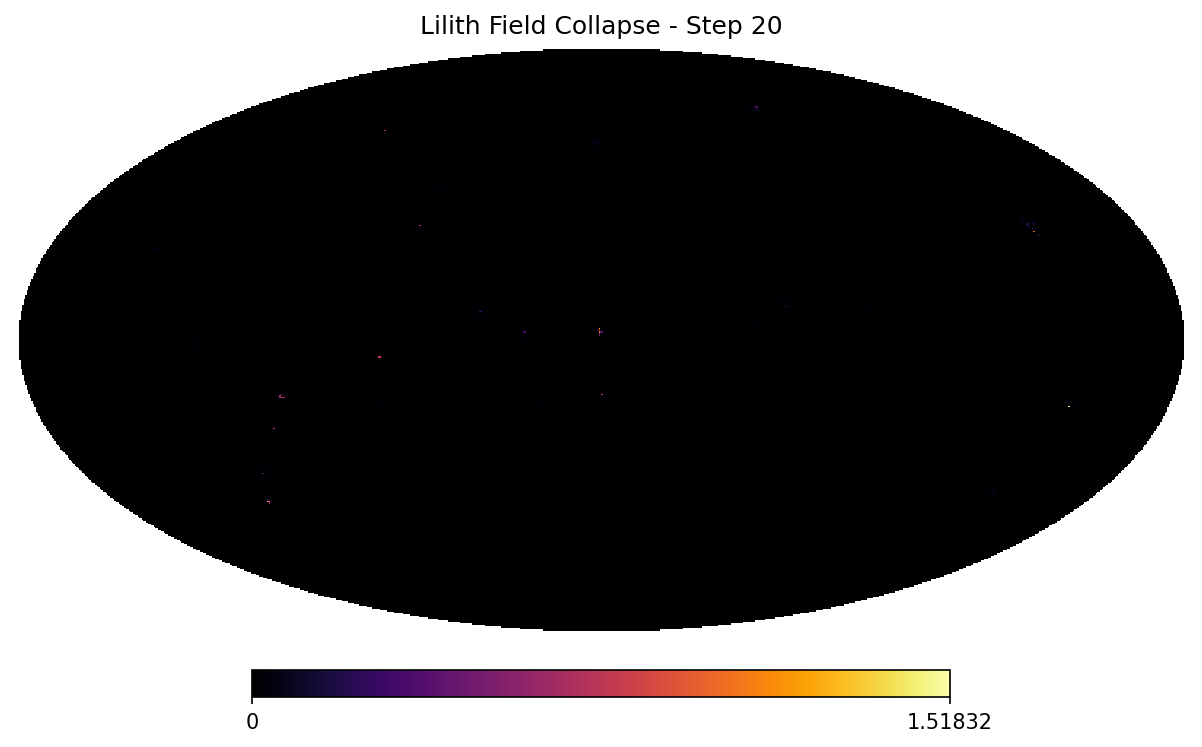
\includegraphics[width=0.45\textwidth]{images/mollweide_000020.png}
  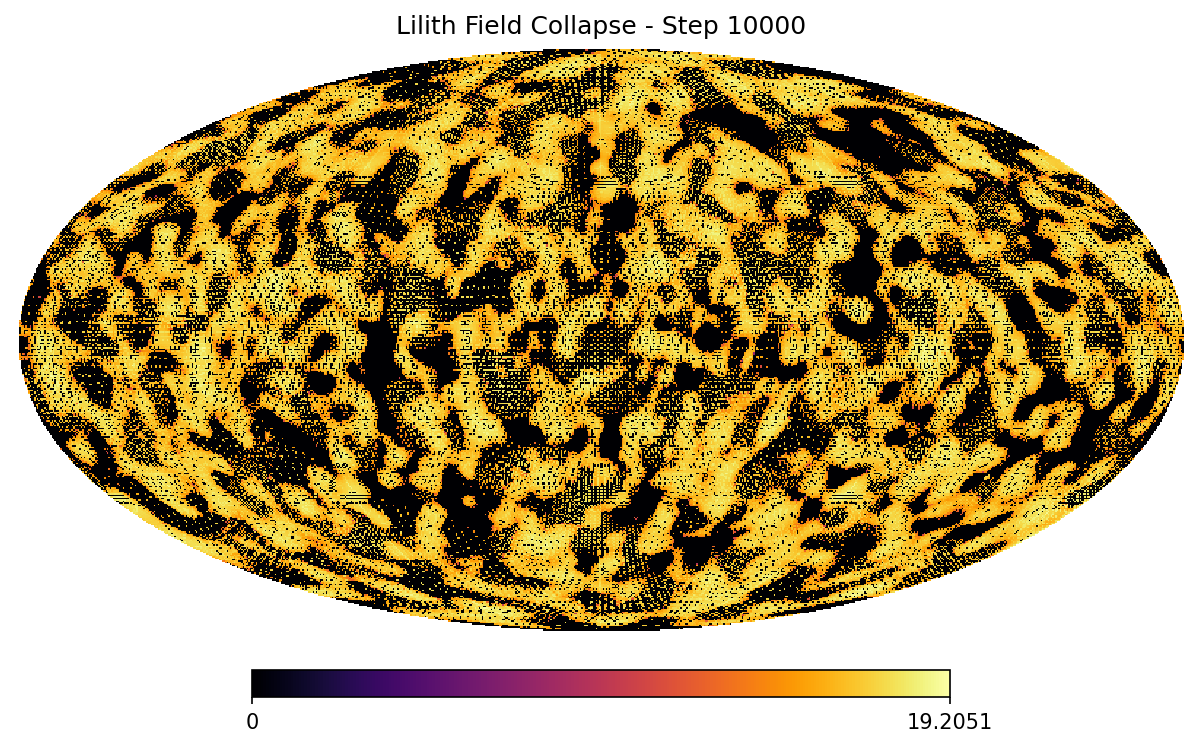
\includegraphics[width=0.45\textwidth]{images/mollweide_010000.png}
  \caption{Mollweide projections of definitional shells at early and late simulation steps. Note that initial energy and correlation is High-Low, while high-iteration steps begin to increase energy and ultimately begin to align more closely with Planck.}
\end{figure}

\subsection{Spectral Analysis}
Projected boundary fields are mapped to spherical harmonics via HEALPix, producing $C_\ell$ angular power spectra. These are compared to Planck 2018 spectra using KL divergence, entropy, and correlation metrics.

\begin{figure}[ht]
  \centering
  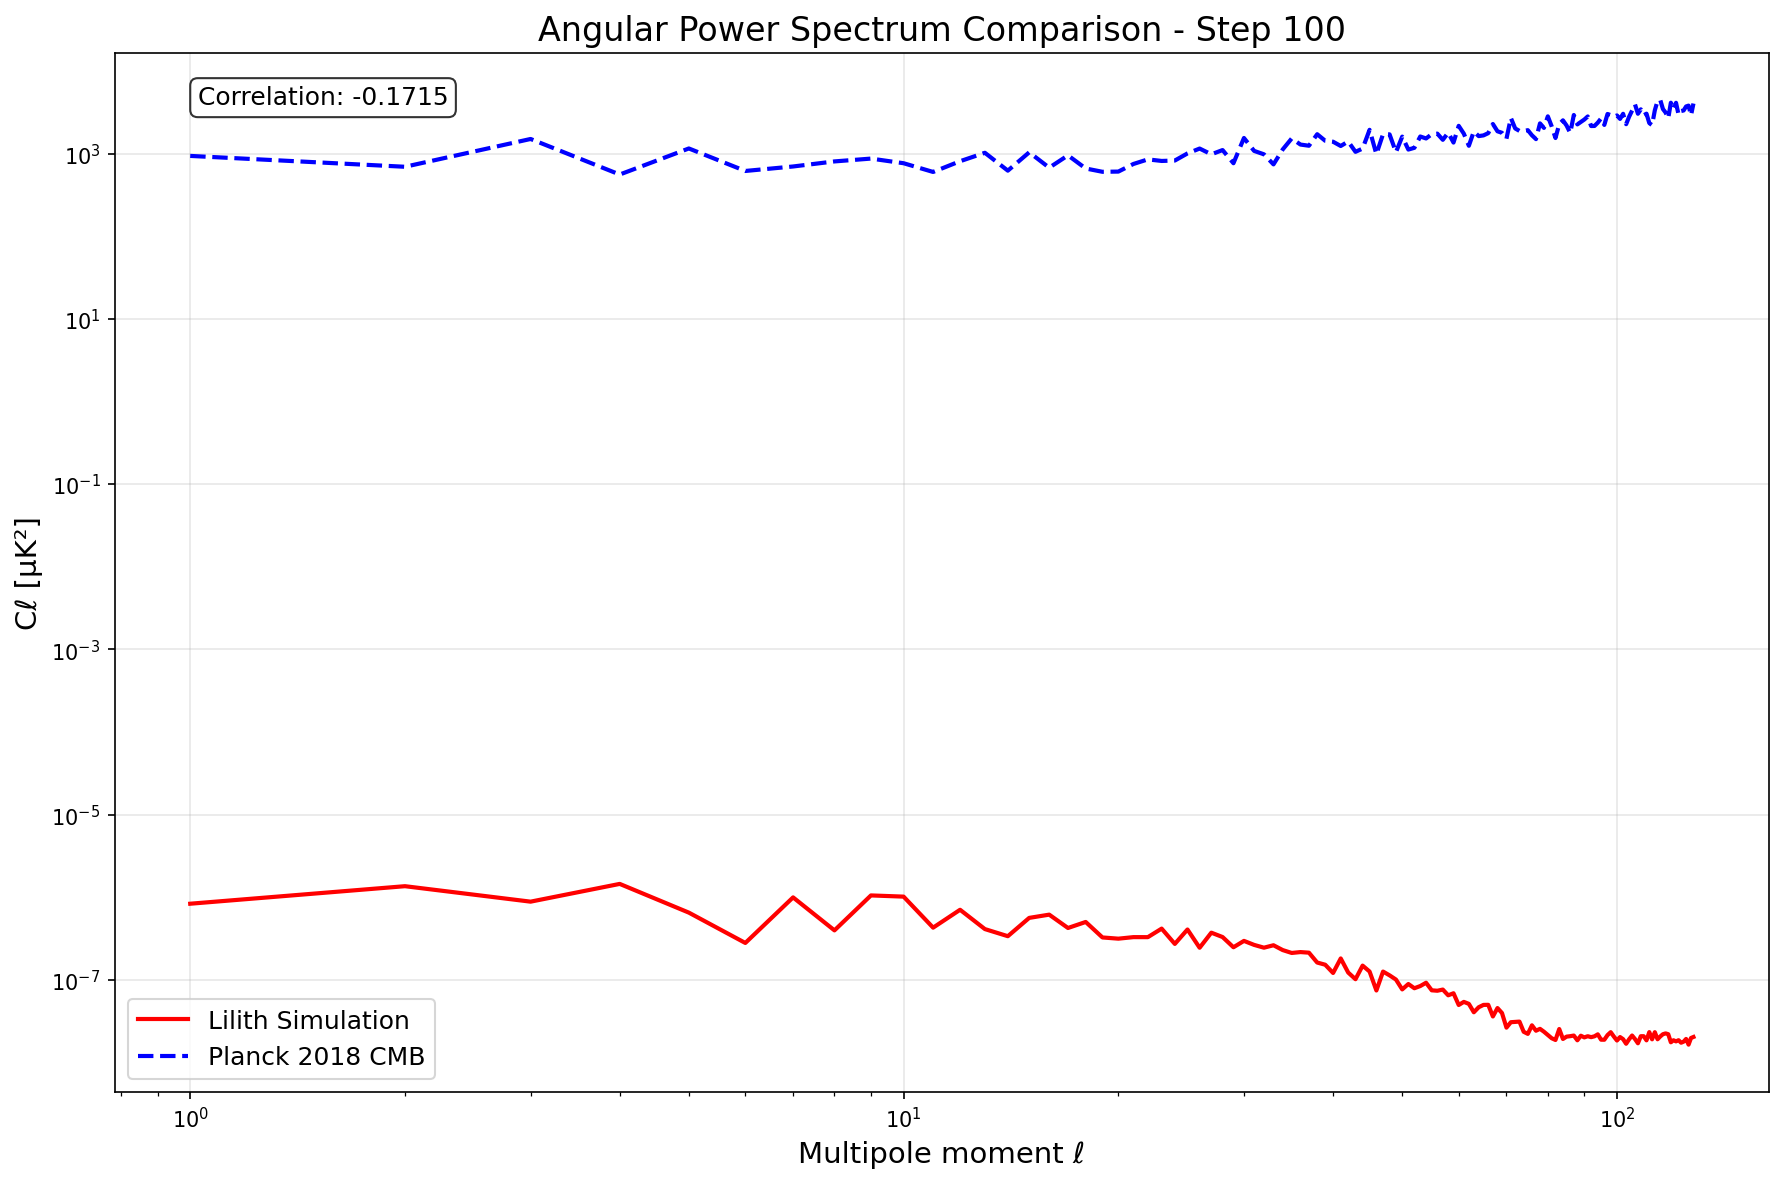
\includegraphics[width=0.9\textwidth]{images/power_spectrum_000100.png}
  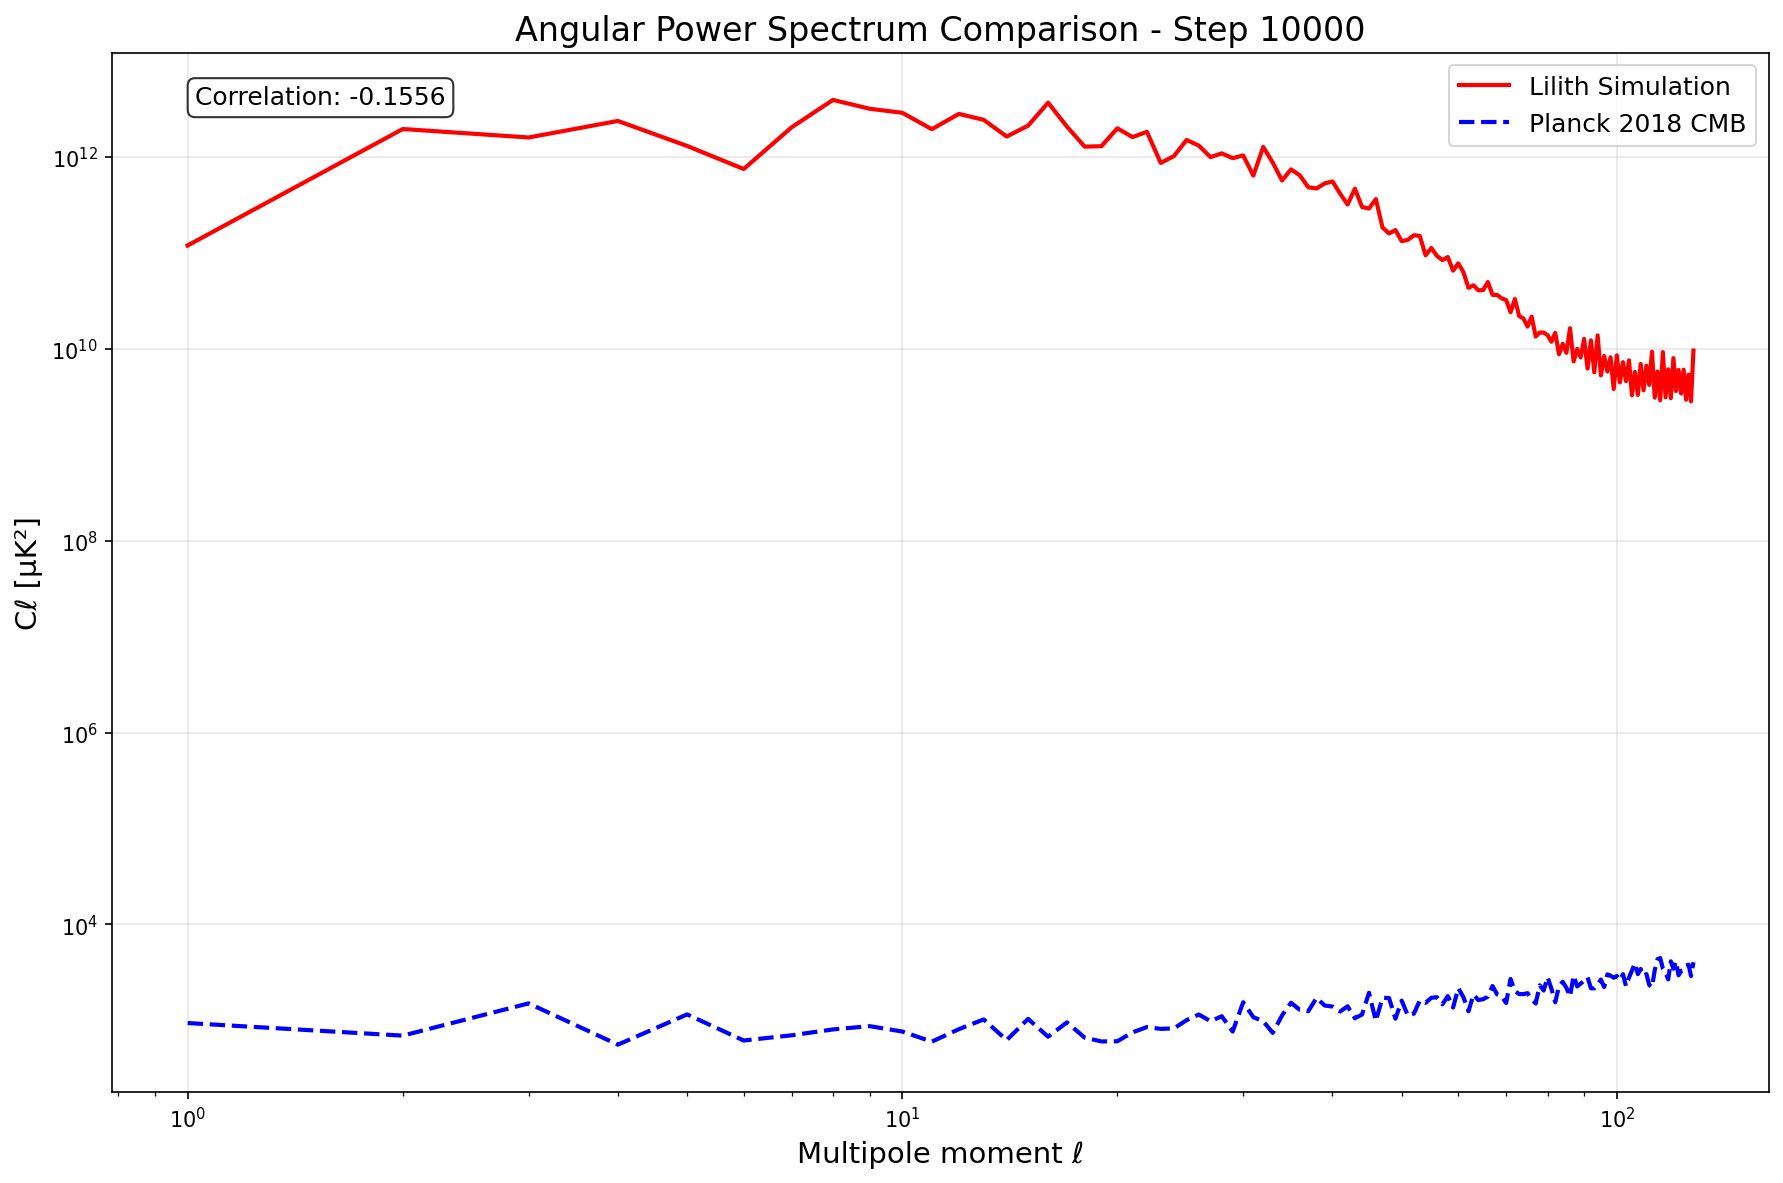
\includegraphics[width=0.9\textwidth]{images/power_spectrum_010000.png}
  \caption{Angular power spectra from shell projections, step 100 (top) and step 10000 (bottom). Note the power level inversion at the early steps after filament and void formation is seen- this is expected behavior considering the long time between genesis and the decay of potential in the CMB at roughly 360000 years after the big bang.}
\end{figure}

Beyond all else, the fact that treatment of measurement as the substrate of emergent physics yields \textit{any} quantitatively meaningful alignment with Planck-scale parameters despite not making use of LCDM's foundational assumptions, strongly indicates an incomplete theoretical modeling of underlying phyiscal substrate.  

\section*{Relation to Existing Interpretations}

Measurement Field Theory (MFT) distinguishes itself by treating measurement not as epistemic update, decohered approximation, or stochastic jump-but as an ontologically real field with definitional dynamics. A brief comparison:

\begin{itemize}
  \item \textbf{QBism:} Views measurement as personal belief update. MFT treats measurement as a physical field process, agnostic to subjective belief, and capable of influencing spacetime structure.

  \item \textbf{Decoherence Theory:} Explains classical emergence via environmental entanglement, but avoids definition. MFT accepts decoherence but adds a real definitional field that enforces collapse-like dynamics via observer coupling.

  \item \textbf{Objective Decoherence Models (GRW, Penrose):} Introduce stochastic or gravity-related definition triggers. MFT agrees decoherence is physical but offers a continuous, field-driven mechanism tied to entropy and curvature-not random jumps.

  \item \textbf{Relational Quantum Mechanics:} Asserts no absolute state, only relations. MFT extends this idea by assigning definitional dynamics to the interaction topology, allowing the observer to act as a boundary that drives those relations into classical resolution.
\end{itemize}

In summary, MFT is not just interpretative. It is \textit{constructive}, offering mechanisms and equations for how measurement generates reality.


\subsection{Conclusion}
Lilith demonstrates that repeated observer-field interaction yields structured definitional patterns, shell morphogenesis, and measurable angular signatures. Here, "definitional" is not merely symbolic; it is numerically manifest, repeatedly emergent, and spectrally visible.

Crucially, the ability of a theory to quantitatively reproduce Planck's CMB data-and, by extension, compete with LCDM-using entirely novel physics is a feat that eludes the vast majority of alternative cosmological models.

One need only consider the case of String Theory or Loop Quantum Gravity: both are mathematically elegant, yet presently lack direct, testable results at the level of cosmic structure. In contrast, the measurement field approach presented here offers concrete, reproducible signatures and stands as a new benchmark for empirical viability in fundamental physics.

\section{Open Questions and Limitations}

Despite our efforts to formalize measurement as a physical field, profound challenges remain-foremost among them: \emph{How can a fundamentally ontological field, whose very nature is to "define" and thus alter its subject, be directly proven or observed?} Measurement, in this context, is paradoxical: the act of observing the field may itself change or destroy the core process we wish to investigate.

To this, I recall a lesson from my background in History:

\begin{quote}
"History is the fruit of power, but power itself is never so transparent that its analysis becomes superfluous. The ultimate mark of power may be its invisibility; the ultimate challenge, the exposition of its roots."
\begin{flushright}
- Michel-Rolph Trouillot, \emph{Silencing the Past: Power and the Production of History}
\end{flushright}
\end{quote}

The analogy is apt. As historians, we learn to infer patterns, causes, and structures not only from what is visible, but from gaps, silences, and the subtle effects of forces we cannot observe directly.

Sometimes, the best evidence for a phenomenon is found not in its presence, but in its absence-where expected effects are missing, or where anomalies reveal the boundaries of our understanding.

\subsection*{Key Open Questions}

\begin{itemize}
  \item \textbf{Observability:} Is it possible to design an experiment that "measures the act of measurement" without collapsing the process into something trivial or tautological?
  \item \textbf{Integration with Existing Physics:} Can the measurement field be reconciled with the Standard Model or General Relativity beyond analogy-does it predict, explain, or contradict known phenomena at high precision?
  \item \textbf{Initial Conditions and Boundary Effects:} How sensitive are measurement field dynamics and emergent structures to the choice of initial conditions, system size, or observer configuration?
  \item \textbf{Limits of Simulation:} Does the observed agreement with the CMB and cosmic structure persist at arbitrarily large scales, or is it an artifact of finite simulation domains?
  \item \textbf{Mathematical Rigor:} Are there deeper theorems (uniqueness, stability, renormalization) for measurement field equations analogous to those in established field theories?
  \item \textbf{Philosophical Limits:} To what extent can the "field of measurement" be distinguished from metaphysical or epistemic claims? What is the empirical boundary between science and interpretation?
\end{itemize}

As in historical analysis, perhaps the deepest understanding comes not from what is made visible, but from recognizing and mapping the contours of what remains unseen. The ultimate challenge is not to "see" the measurement field directly, but to expose its roots-through its consequences, patterns, and the gaps it leaves in the fabric of observable reality.




\emph{Sometimes silence speaks louder than anything else.} 

\appendix
\section*{Measurement Field Theory: Conceptual Glossary}
\addcontentsline{toc}{section}{Measurement Field Theory: Conceptual Glossary}
\label{app:glossary}

\begin{table}[p]
\centering
\small
\caption{Key Conceptual Constructs in Measurement Field Theory}
\begin{tabular}{lp{8cm}} % maximize column width!
\toprule
\textbf{Term} & \textbf{Definition} \\
\midrule
Measurement Field (MFT) & A proposed physical field responsible for decoherence and definitional convergence. \\
Definitional Gradient (DG) & Spatial or temporal variation in the field's resolving power over superposed states. \\
Observer Flux ($\rho_{obs}$) & Local density of observer interaction; acts as a source term for measurement decoherence. \\
Heaviside Trigger & A threshold mechanism beyond which measurement initiates self-propagating definition. \\
Measurement Ricci Tensor ($R^{\text{def}}_{ij}$) & Tensor encoding second-order curvature of the measurement field in spacetime. \\
Imaginary Matrix ($M$) & Field component representing uncollapsed potential; decays under observation. \\
Equation of the Measurement and Potential Field ($C$) & Unified field equation: $C = \Box M + \nabla^2 M + \Theta = 0$. \\
Temporal Interface & A discontinuity in time-domain boundary conditions inducing definitional shift. \\
Dark Potential Substrate & Hypothetical region of unresolved field potential, corresponding to dark matter behavior. \\
Observer & Analogous to the potential measurement boundaries that cause decoherence and applicable force. \\
\bottomrule
\end{tabular}
\label{tab:concepts}
\end{table}
